\documentclass[tikz,border=10pt]{standalone}
\usepackage{amsmath}
\usetikzlibrary{arrows.meta, positioning, calc, decorations.pathreplacing}
\definecolor{c1}{HTML}{000000}
\definecolor{c2}{HTML}{233D4D}
\definecolor{c3}{HTML}{FE7F2D}
\definecolor{c4}{HTML}{EAECF0}
\definecolor{axiscolor}{HTML}{333333}
\definecolor{labelcolor}{HTML}{5F6B75}
\begin{document}
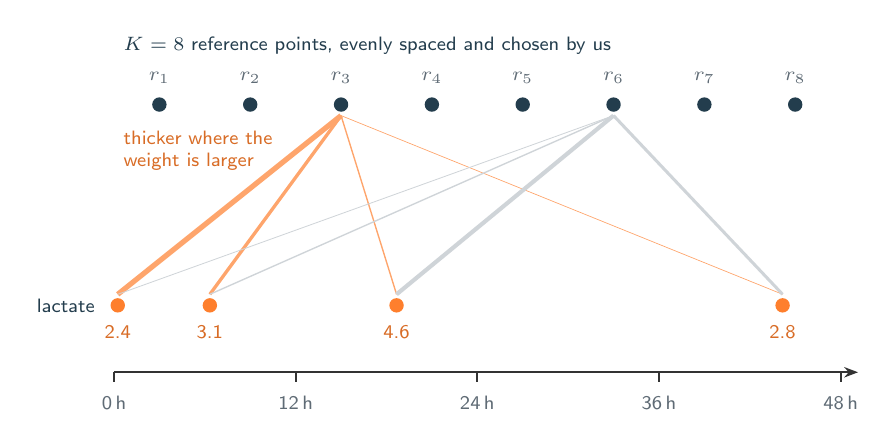
\begin{tikzpicture}[
    every node/.style={font=\sffamily},
    lab/.style={font=\sffamily\scriptsize, text=labelcolor},
    tag/.style={font=\sffamily\scriptsize, text=c2},
    hot/.style={font=\sffamily\scriptsize, text=c3!85!black},
]
\def\X#1{1.70 + #1*0.003200}

% ---------------- reference points on top
\node[tag, anchor=west] at (1.70, 5.35) {$K = 8$ reference points, evenly spaced and chosen by us};
\foreach \k in {0,...,7}{
    \pgfmathsetmacro\m{180 + \k*360}
    \fill[c2] ({\X{\m}}, 4.60) circle (2.6pt);
    \pgfmathtruncatemacro\kk{\k+1}
    \node[lab, anchor=south] at ({\X{\m}}, 4.74) {$r_{\kk}$};
}

% ---------------- observations below
\node[tag, anchor=east] at (1.58, 2.05) {lactate};
\foreach \m/\v in {15/2.4, 380/3.1, 1120/4.6, 2650/2.8}{
    \fill[c3] ({\X{\m}}, 2.05) circle (2.6pt);
    \node[hot, anchor=north] at ({\X{\m}}, 1.92) {\v};
}

% ---------------- weighted edges from one reference point
\foreach \m/\w in {15/1.9, 380/1.2, 1120/0.5, 2650/0.25}{
    \draw[c3!70, line width=\w pt] ({\X{900}}, 4.46) -- ({\X{\m}}, 2.19);
}
\node[hot, anchor=west, align=left] at (1.70, 4.02) {thicker where the\\ weight is larger};

% a second, fainter fan
\foreach \m/\w in {15/0.3, 380/0.5, 1120/1.5, 2650/1.1}{
    \draw[c2!22, line width=\w pt] ({\X{1980}}, 4.46) -- ({\X{\m}}, 2.19);
}

\draw[axiscolor, line width=0.8pt, -{Stealth[length=5pt]}] (1.70, 1.20) -- (11.15, 1.20);
\foreach \h in {0, 12, 24, 36, 48}{
    \pgfmathsetmacro\m{\h*60}
    \draw[axiscolor, line width=0.7pt] ({\X{\m}}, 1.20) -- ({\X{\m}}, 1.08);
    \node[lab, anchor=north] at ({\X{\m}}, 1.02) {\h\,h};
}
\end{tikzpicture}
\end{document}
